\chapter{Bilan du projet}

\section{Autocritique}
Nous avons pu valider quatre fonctionnalités parmi celles qui étaient prévues au départ dans le cahier des charges.
\begin{itemize}
\item Créer le moteur de jeu de rythme avec Unity, et un jeu l'utilisant
\item Rendre l'application jouable sur tous les supports
\item Créer d'autres mini-jeux utilisant le moteur
\item Créer un moteur de tutoriels, et créer les tutoriels pour les jeux
\end{itemize}

Les trois premières fonctionnalités sont les plus importantes et donc nécessaires à la réussite du projet. Elles ont étés implémentées avec succès.

\paragraph{}
Cependant, plusieurs idées initiales ont du être abandonnées en cours de projet. Le principe de la "planète d'accueil" que le joueur devait personnaliser grâce aux objets qu'il aurait gagné dans les mini-jeux, ainsi que le niveau qui se joue à l'infini, n'ont pas étés développés. En effet, après avoir réalisé l'ampleur de la tâche que représentait la création d'un seul mini-jeu, de sa conception, jusqu'à son intégration finale avec le moteur, nous avons décidé de nous impliquer pleinement dans ce processus afin d'obtenir des mini-jeux ergonomiques et cohérents pour un utilisateur. C'est ainsi que plusieurs prototypes de mini-jeux n'ont pas dépassé le stade de la conception car jugés peu compréhensibles pour le type de gameplay facile et amusant que nous désirions.

\begin{figure}[H]\centering
   \begin{minipage}{0.49\textwidth}\centering
     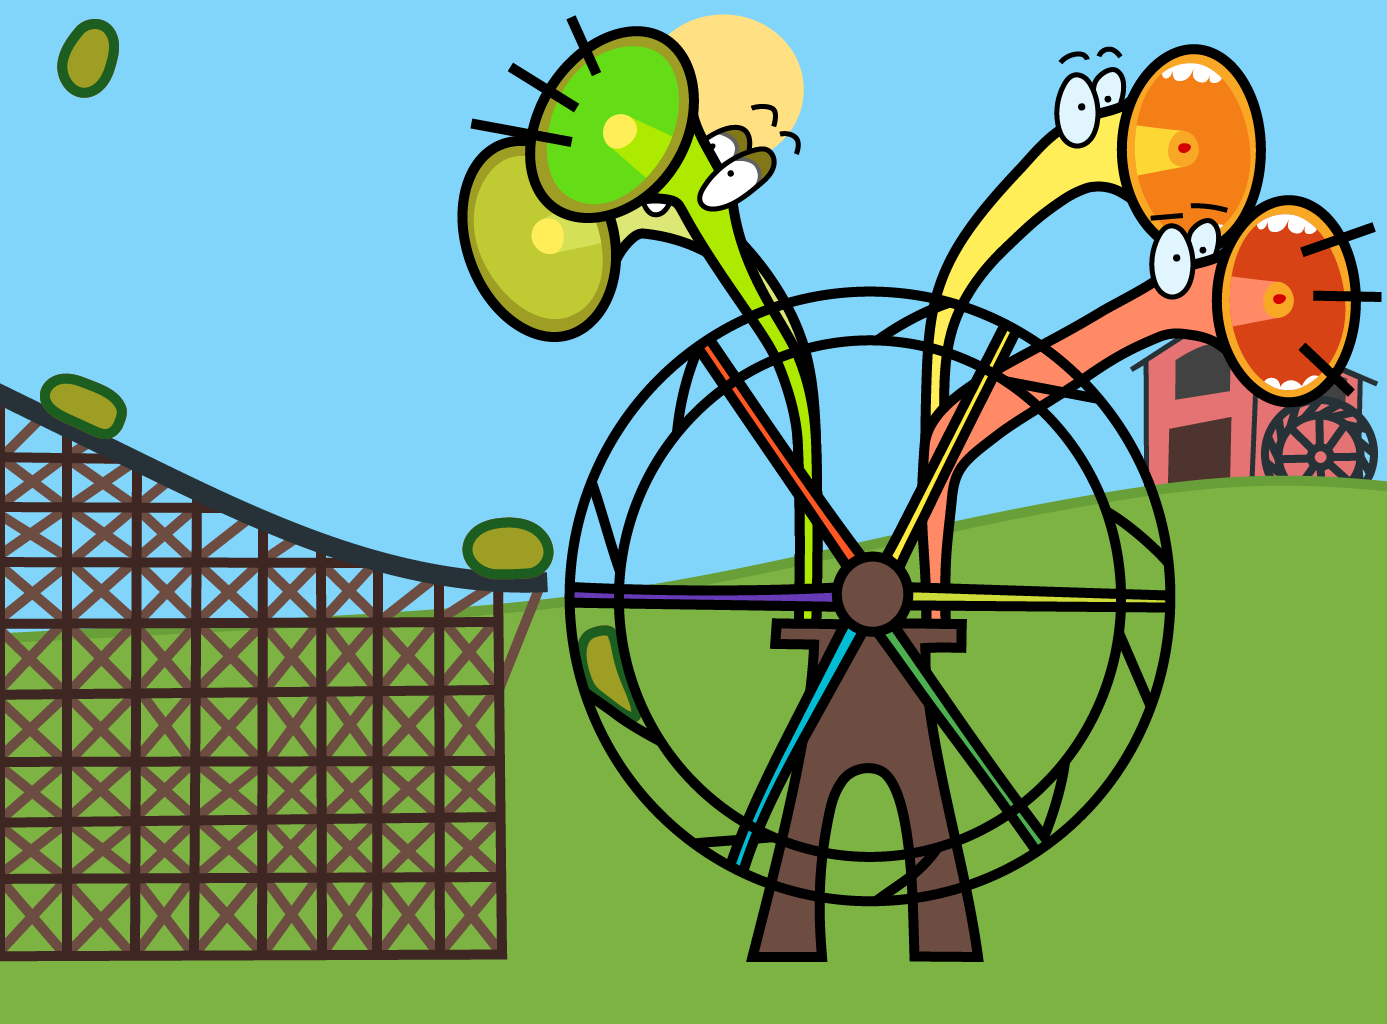
\includegraphics[scale=0.1]{./img/concept_moulin.png}
     \caption{Concept du jeu du moulin}
     \label{jeu_concept1}
   \end{minipage}
   \begin {minipage}{0.49\textwidth}\centering
     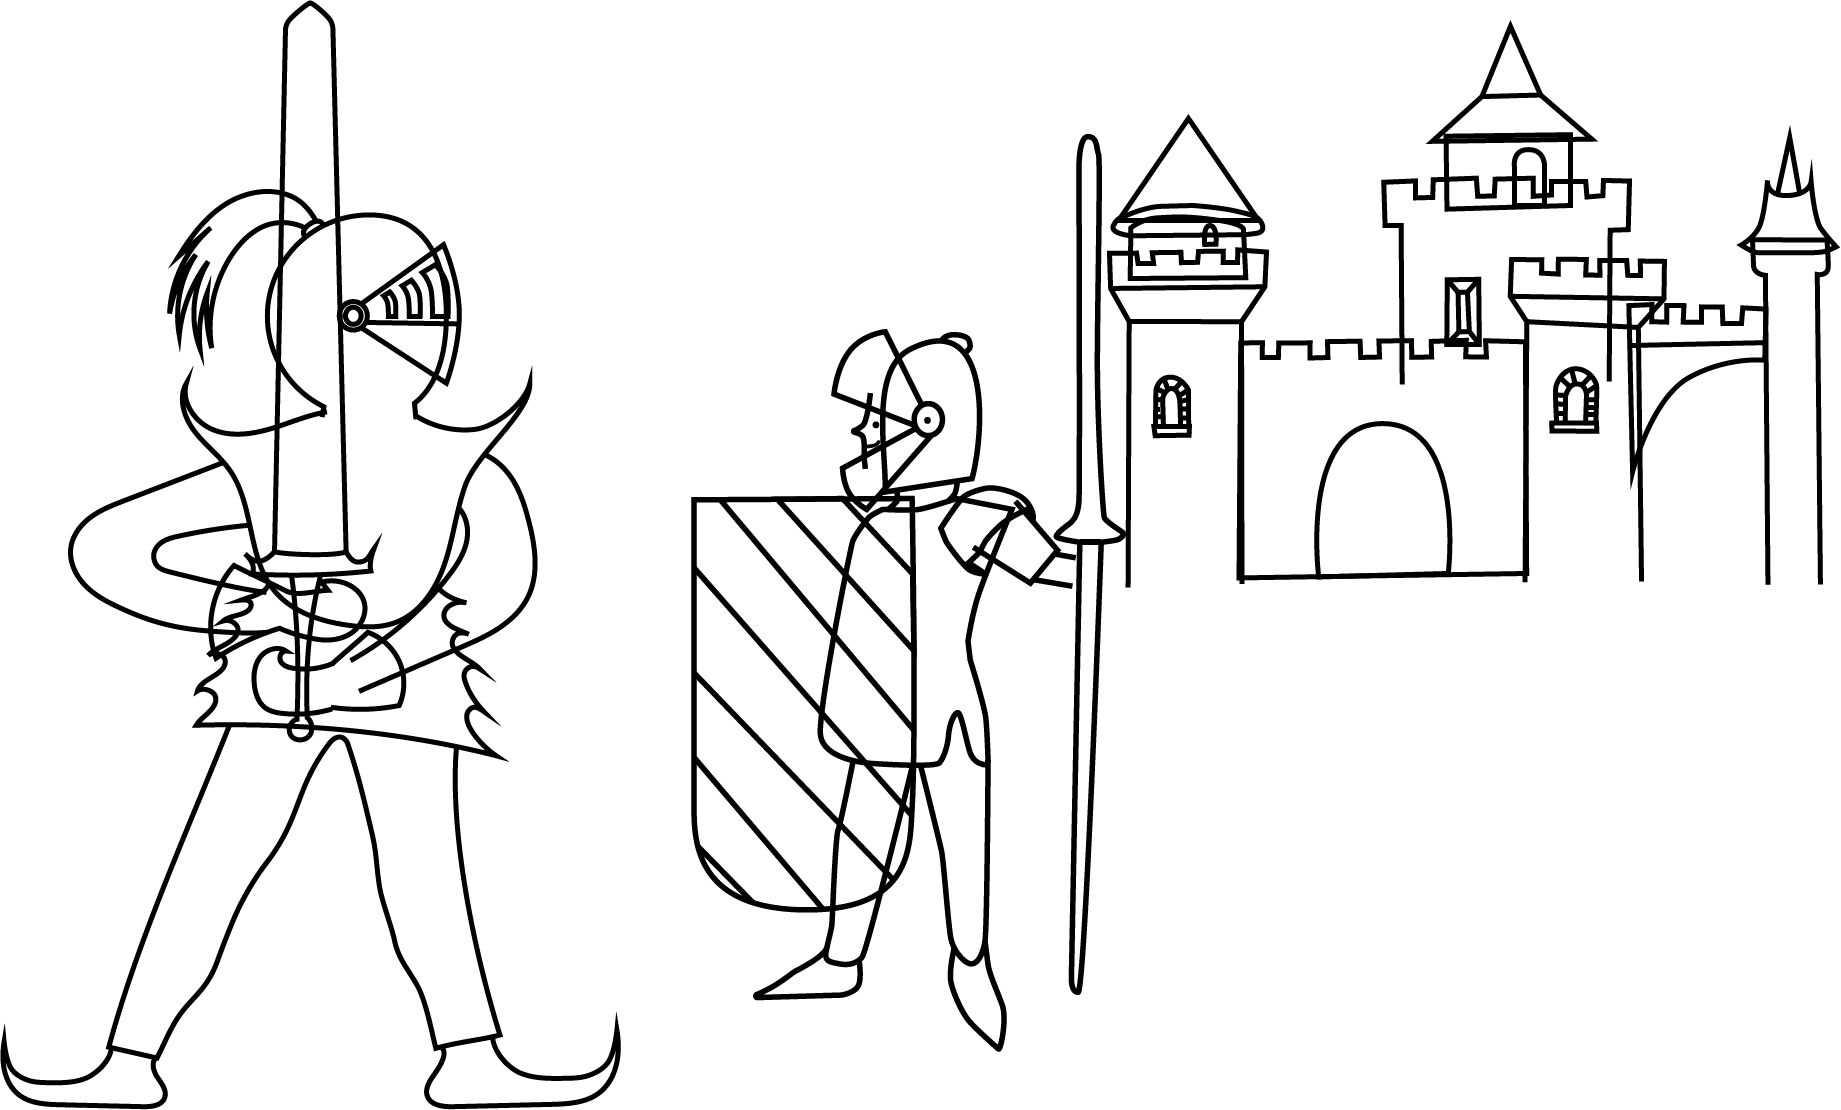
\includegraphics[scale=0.1]{./img/concept_chevalier.png}
     \caption{Concept d'un jeu de chevaliers}
     \label{jeu_concept2}
   \end{minipage}
\end{figure}

\paragraph{}
Le principal objectif que nous nous étions fixés au sein du groupe, était d'avoir une application fonctionnelle, propre, bien codée et en ligne. Cet objectif est accompli, l'application est fonctionnelle et présente sur les marchés d'applications pour les systèmes Android et Apple.

\section{Enseignements tirés}


\section{Perspectives}


\section{Conclusion}

